\documentclass[a4paper, 12pt]{article}

\usepackage[utf8]{inputenc}
\usepackage[spanish,es-noquoting]{babel}
\usepackage{enumitem}
\usepackage[a4paper,bindingoffset=0.2in,%
            left=1in,right=1in,top=1in,bottom=1in,%
            footskip=.25in]{geometry}
\linespread{1.25}

\usepackage{graphicx}
\usepackage{hyperref}
\usepackage{pdfpages}
\usepackage{pdflscape}



\title{Plan de Trabajo}
\author{Alejandro García Castellanos\\z17m008}

\tolerance=1
\emergencystretch=\maxdimen
\hyphenpenalty=10000
\hbadness=10000


\begin{document}
\maketitle 

\section{Descripción general del trabajo}
El trabajo se basa en el estudio y exposición del Teorema de estabilidad, el cual, a grandes rasgos, establece que pequeñas perturbaciones en los datos implican pequeñas perturbaciones en la homología persistente. Para ello me centraré en el siguiente artículo: \textit{\href{https://link.springer.com/content/pdf/10.1007/s00454-006-1276-5.pdf}{Cohen-Steiner, David \& Edelsbrunner, Herbert \& Harer, John. (2005). Stability of Persistence Diagrams. Discrete \& Computational Geometry - DCG. 37. 263-271. 10.1007/s00454-006-1276-5}}.\\

Adicionalmente, implementaré en Python la distancia \textit{Bottleneck} para poder ilustrar este teorema haciendo uso distintos conjuntos de datos. La implementación se sustenta en el uso de complejos simpliciales y su correspondiente homología simplicial.

\subsection*{Objetivos}
\begin{itemize}
	\item Buscar referencias que contengan el enunciado y la demostración del Teorema de estabilidad.
	\item Estudiar y entender estas referencias.
	\item Implementar el cálculo de la distancia de Bottleneck entre diagramas de persistencia.
	\item Ilustrar el Teorema de estabilidad sobre distintos conjuntos de datos.
	\item Redactar la memoria y preparar la presentación
\end{itemize}

\section{Tareas}
Es por ello que las principales tareas para la realización del trabajo son:
\begin{itemize}
	\item \textbf{Preparación}
	\begin{itemize}
		\item Buscar referencias que contengan el enunciado y la demostración del Teorema de estabilidad.
		\item Repasar los contenidos de la asignatura de Topología Computacional.
	\end{itemize}
	
	\item \textbf{Realización de los objetivos principales}
	\begin{itemize}
		\item Estudiar y entender estas referencias.
		\item Implementar el cálculo de la distancia Bottleneck entre diagramas de persistencia
		\begin{enumerate}
			\item Búsqueda de los algoritmos.
			\item Implementación sobre clase de complejos simpliciales programada en la asignatura de Topología Computacional.
			\item Testing de las nuevas funcionalidades.
		\end{enumerate}
	\end{itemize}
	
	\item \textbf{Elaboración de la Memoria y Presentación}
	\begin{itemize}
		\item \textbf{Memoria}
		\begin{itemize}
			\item Redactar conocimientos previos requeridos para la comprensión del teorema.
			\item Redactar Teorema de estabilidad y su demostración
			\item Ilustrar el teorema a través de su implementación.
		\end{itemize}
		\item Elaboración y preparación de la presentación.
	\end{itemize}
	
\end{itemize}

\section{Copia de la propuesta de trabajo escrito por el tutor}

El Análisis Topológico de Datos es una disciplina que utiliza técnicas de topología algebraica para extraer información global sobre grandes cantidades datos. Es una disciplina que ha tenido un gran desarrollo desde los años 90 hasta nuestros días. La herramienta fundamental para este tipo de estudio es la homología persistente. Uno de los resultados más importantes sobre la homología persistente es el célebre Teorema de estabilidad que, grosso modo, establece que pequeñas perturbaciones en los datos implican pequeñas perturbaciones en la homología persistente.

El objetivo fundamental de este trabajo es estudiar, entender y exponer este resultado y su demostración además de implementar el cálculo de la distancia Bottleneck entre diagramas de persistencia para poder ilustrar este resultado con diversos ejemplos.

\section{Diagrama Gannt}

\begin{landscape}
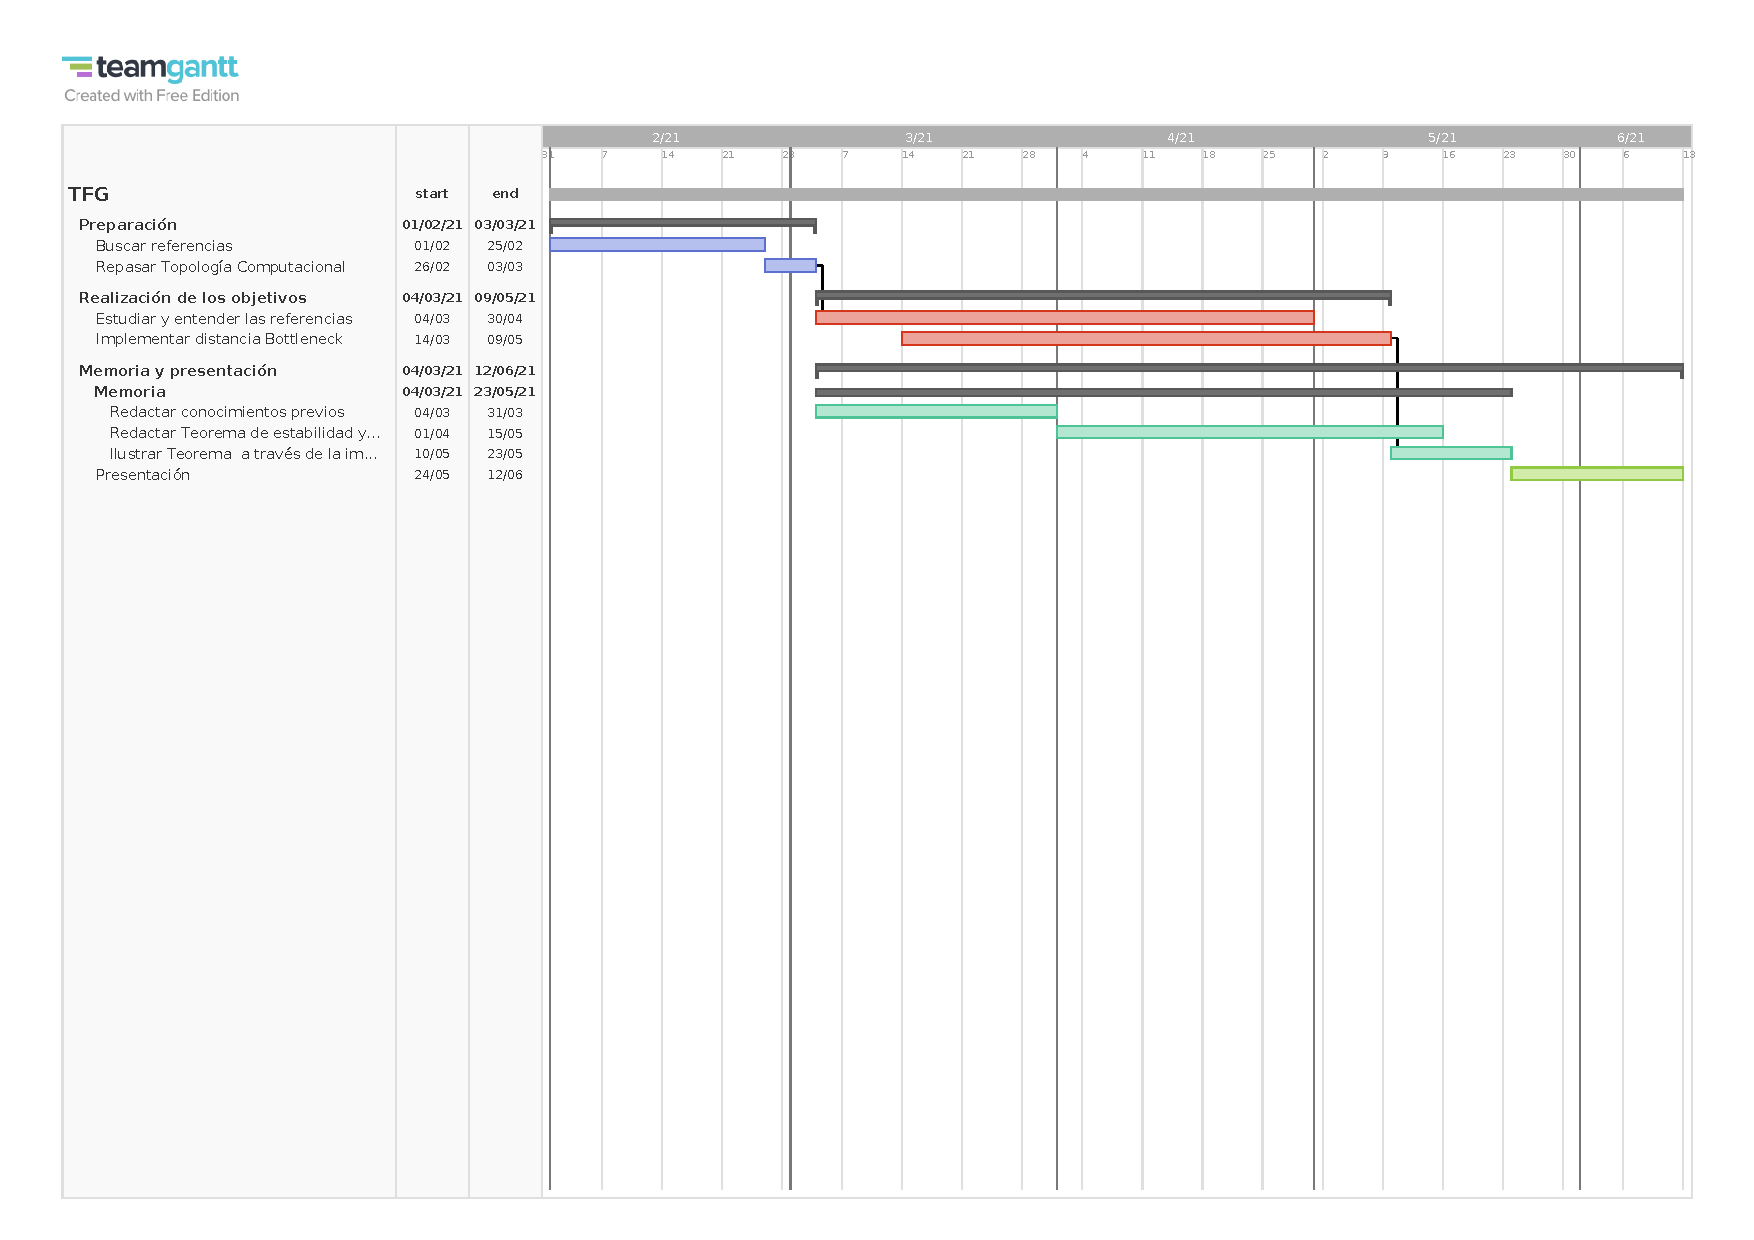
\includepdf[landscape=true, landscape]{TFG_gantt}
\end{landscape}


\end{document}





